\section{Finite Differencing}
%
\paragraph{Hemispheric symmetry}
%
As mentioned in section \ref{cap:electro_equ} we assume that the conductivity 
along the magnetic field line is
very large such that conjugate foot points are equipotential. To get a symmetric
potential pattern we add the two hemispheres together and solve for only one
hemisphere. The symmetrie of the potentail pattern is only valid at low-- and
mid--latitudes. At high latitudes the electric potential is specially treated as
discussed in section \ref{cap:high_lat}. \\
%
The added values are denoted by $(\cdot)^T$ and are summarized in equation 
(\ref{eq:nh_1})--(\ref{eq:nh_6}). In the source code 
\texttt{subroutine dynamo} the following values are calculated
%
\begin{align}
   \Sigma_{\phi \phi}^T(0)      = \Sigma_{\phi \phi}^{NH}(0) + \Sigma_{\phi \phi}^{SH}(0)\\
   \Sigma_{\lambda \lambda}^T(0)=\Sigma_{\lambda \lambda}^{NH}(0)+ \Sigma_{\lambda \lambda}^{SH}(0) \\
  -\Sigma_{C}^T(0)= -(\Sigma_{C}^{NH}(0)-\Sigma_{C}^{SH}(0))\\
   \Sigma_{H}^T(0)=   \Sigma_{H}^{NH}(0)-\Sigma_{H}^{SH}(0)\\
   K_{m \phi}^{DT}(0)    = K_{m \phi}^{D,NH}(0)+ K_{m \phi}^{D,SH}(0)\\
   K_{m \lambda}^{DT}(0) = K_{m \lambda}^{D,NH}(0)-K_{m \lambda}^{D,SH}(0)
\end{align}
%
Note that in the source code $-\Sigma_{C}^T(0)$ is put into ZIGMC, and that
$-K_{m \lambda}^{D,SH}(0)$ is saved in RIM(2). These values are saved in the latitude indices of
the northern hemisphere from $nmlat+1/2$ which is the index for the equator to
the pole at $nmlat$. $nmlat$ are the numbers of magnetic latitudes.
%
\paragraph{Differencing of the right hand side}
%
In \texttt{subroutine rhspde} the right hand side is differentiated. 
%
\begin{equation}
   rhs = \frac{1}{cos \lambda_0} \bigl[ R_0 \frac{\partial K_{m \phi}^{DT}(0)}{\partial \phi_0} +  
   R_0 \frac{\partial K_{m \lambda }^{DT}(0) cos \lambda_0}{\partial | \lambda_0 |}
   \bigr] \label{eq:diff_rhs}
\end{equation}
%
A central differencing scheme is used which lead to the derivative at the location 
$\phi(i)$, $\lambda_0(j)$ to
%
\begin{equation}
\begin{split}
  rhs(i,j) = & \frac{1}{ 2 \Delta \phi cos \lambda_0(j)} \bigl[ K_{m \phi}^{DT}(0)(i+1,j) - 
      K_{m \phi}^{DT}(0)(i-1,j)\bigr] + \\
   & \frac{1}{ 2 \Delta \lambda_0 cos \lambda_0(j)} \bigl[ K_{m \lambda }^{DT}(0)(i,j+1) 
    cos \lambda_0(j+1)- K_{m \lambda }^{DT}(0)(i,j-1)cos \lambda_0(j-1) \bigr] 
\end{split}
\end{equation}
%
with i,j the longitudinal and latitudinal index and the adjacent points $i\pm 1$,$j \pm1$.
The polar derivative is approximated by
%
\begin{equation}
   rhs (i,j_{pole}) = - \frac{2}{cos \lambda_0(j-1) mlon} \bigl[ \sum_{i=1}^{mlon} 
       K_{m \lambda }^{DT}(0)(i,j_{pole} - 1)  \bigr]
\end{equation}
%
At the geomagnetic equator the $cos \lambda_0(j_eq)=1$ and $K_{m \lambda }^{DT}(0)(i,j_eq) =0$.
Therefore the derivative with respect to $\lambda_0$ which is
%
\begin{equation}
  \frac{2}{ \Delta \lambda_0} \bigl[ K_{m \lambda }^{DT}(0)(i,j_{eq}+
       \frac{1}{2}) - K_{m \lambda }^{DT}(0)(i,j_{eq}) \bigr]
\end{equation}
%
reduces to 
%
\begin{equation}
  \frac{2}{ \Delta \lambda_0} \bigl[ K_{m \lambda }^{DT}(0)(i,j_{eq}+
       \frac{1}{2})  \bigr]
\end{equation}
%
with $ K_{m \lambda }^{DT}(0)(i,j_{eq}+ \frac{1}{2} =  1/2 [K_{m \lambda }^{DT}(0)(i,j_{eq}) +
K_{m \lambda }^{DT}(0)(i,j_{eq}+ 1)] $. The derivative at the geomagnetic equator can be written
as 
%
\begin{equation}
\begin{split}
  rhs(i,j_{eq}) =& \frac{1}{ 2 \Delta \phi cos \lambda_0(j)} \bigl[ K_{m \phi}^{DT}(0)(i+1,j) - 
      K_{m \phi}^{DT}(0)(i-1,j)\bigr] + \\
     &\frac{1}{ \Delta \lambda_0 } \bigl[ K_{m \lambda }^{DT}(0)(i,j_{eq}+1) 
    cos \lambda_0(j_{eq}+1)+ K_{m \lambda }^{DT}(0)(i,j_{eq})cos \lambda_0(j_{eq}) \bigr]  
\end{split}
\end{equation}
%
The whole right hand side is muliplied by $R_0$ in [m] to get eq. (\ref{eq:diff_rhs}). 
%
\paragraph{Differencing of the left hand side}
%
In this paragraph the finite differencing of the left hand side is
discussed. In the source code the calling tree for the differencing is the
following:
%
\begin{verbatim}
subroutine dynamo
if isolve = 2 then
   call stencmd
        call htrpex
        call cnmmod
        call cnm
else
   call stencil
        call htrpex
        call cnm
endif
\end{verbatim}
%
Note that the ditinction between the flag \flags{isolve} is due to the
solving algorithm of the electrodynamo equation with the multigrid
solver. The flag  \flags{isolve}=2 means that at the finest grid the
coefficient matrix is set up without upwinding for terms where
the diagonal dominance is violated (see paragraph further down in this section). Upwinding
is used at all grid levels for \flags{isolve}$ \neq 2$. For more information
about the multigrid solver we refer to section \ref{cap:solve}. \\
 
%
In \texttt{subroutine dynamo} the coefficients are prepared for the
finite differencing. The coefficients represent 
% 
\begin{align}
A= \frac{\Sigma_{phi phi}^T(0)}{cos\lambda_0  \Delta \phi^2 }	   \rightarrow  zigm11\label{eq:sig_dif1}\\
B= \frac{\Sigma_{lam lam}^T(0) cos \lambda_0)}{\Delta \lambda_0^2} \rightarrow  zigm22\label{eq:sig_dif2} \\
C= \frac{\Sigma_{phi lam}^T(0)}{4\Delta \lambda_0 \Delta \phi }    \rightarrow  zigmc \label{eq:sig_dif3} \\
D= \frac{\Sigma_{phi lam}^T(0)}{4 \Delta \lambda_0 \Delta \phi}    \rightarrow  zigm2 \label{eq:sig_dif4} 
\end{align}
%
Note that the factor of four is introduced due to the 
central differencing. The values are for both hemisphere added 
together and stored in the index range of the "northern hemisphere" ((nmlat+1)/2 to nmlat), with
index staring at the South Pole going to the North Pole.
In the "southern hemisphere" index range (1 to nmlat/2), the same values as in the
northern range ((nmlat+1)/2 to nmlat) are stored except of the two mixed terms which change
sign.
% 
\begin{align}
 zigmc  \rightarrow -\frac{\Sigma_{phi lam}^T(0)}{4\Delta \lambda_0 \Delta \phi } \\
 zigm2  \rightarrow -\frac{\Sigma_{phi lam}^T(0)}{4 \Delta \lambda_0 \Delta \phi} 
\end{align}
%
The polar value of $\frac{\Sigma_{phi phi}^T(0)}{cos\lambda_0  \Delta \phi^2 }$
is set to zero to avoid floating point exception. The polar value is
not used in the electrodynamo equation since the potential at the poles is
prescribed. \\
%
The \texttt{subroutine stencmd} or \texttt{subroutine stencil} is called
for each coefficient $\Sigma$ and updates the stencil for contributions 
of the corresponding $\Sigma$. First the $\Sigma$ is copied into an
array in \texttt{subroutine htrpex} and longitudinal wrap around points for
the longitudinal derivatives are set. Note that there are 5 different grid
levels and therefore there are 16 additional points on either side of the
array. The array stores the values from the equator (index 1) to the pole
(index nmlath). \\
%
The contributions to the stencil from the different $\Sigma$ are
determined in \texttt{subroutine cnmmod} and/or \texttt{subroutine cnm}.
\texttt{Subroutine cnmmod} is called only for the finest grid level
and \flags{isolve}=2 to set
up the coefficient stencil without upwinding method. All the other grid
levels may use upwinding if necessary to set up the stencil. For 
\flags{isolve} $\neq 2$ all the stencils are determined with upwinding methods
if it's necessary and therefore  \texttt{subroutine cnm} is used.
Please read section \ref{cap:solve} for information about the different
solver types.
%
From equation (\ref{eq:edyn3}) and the values in table \ref{tab:transf_quantities}
we get the following left hand side of the electrodynamo equation.
%
\begin{equation}
 cos \lambda_0 lhs=  \frac{\partial}{\partial \phi_0} 
    \bigl( \frac{\Sigma_{\phi \phi}^T(0)}{cos
   \lambda_0} \frac{\partial \Phi}{\partial \phi_0} + 
   \Sigma_{\phi \lambda}^T(0) \frac{\partial \Phi}{\partial \lambda_0} \bigr) +
   \frac{\partial}
   {\partial  \lambda_0 } \bigl( \Sigma_{\lambda \phi}^T(0)
    \frac{\partial \Phi}{\partial \phi_0} + 
   \Sigma_{\lambda \lambda}^T(0) cos \lambda_0 
   \frac{\partial \Phi}{\partial \lambda_0} \bigr)
    \label{eq:edyn4}
\end{equation}
%
Note that the right hand side $rhs$ in equation (\ref{eq:diff_rhs}) is already divided
by $cos \lambda_0$. Replacing 
the following terms
%
\begin{align}
 T_{\phi}=  \frac{\Sigma_{\phi \phi}^T(0)}{cos
   \lambda_0} \frac{\partial \Phi}{\partial \phi_0} + 
   \Sigma_{\phi \lambda}^T(0) \frac{\partial \Phi}{\partial \lambda_0} \\
 T_{\lambda}= \Sigma_{\lambda \phi}^T(0)
    \frac{\partial \Phi}{\partial \phi_0} + 
   \Sigma_{\lambda \lambda}^T(0) cos \lambda_0 
   \frac{\partial \Phi}{\partial \lambda_0} 
\end{align}
%
in equation (\ref{eq:edyn4}) leads to
%
\begin{equation}
 cos \lambda_0 lhs=  \frac{\partial}{\partial \phi_0} T_{\phi}  +
   \frac{\partial}{\partial  \lambda_0 } T_{\lambda}  \label{eq:edyn5}
\end{equation}
%
In the following we will omit flag of the dependence on $\lambda_0$ for
clarity e.g.
$\Sigma_{\phi \lambda}^T(0)$ will become $\Sigma_{\phi \lambda}^T$
Using central differencing for discretization gives
%
\begin{equation}
 cos \lambda_0 lhs=  \frac{T_{\phi}(i+\frac{1}{2},j)-T_{\phi}(i-\frac{1}{2},j)}
 {\Delta \phi_0}   +
   \frac{ T_{\lambda}(i,j+\frac{1}{2})- T_{\lambda}(i,j-\frac{1}{2})}
   {\Delta  \lambda_0 } T_{\lambda}\label{eq:edyn6}
\end{equation}
%
with
%
\begin{align}
\begin{split}
 T_{\phi}(i+\frac{1}{2},j)=&  \frac{\Sigma_{\phi \phi}^T(i+\frac{1}{2},j)}{cos
   \lambda_0(j)} \frac{ \Phi(i+1,j)- \Phi(i,j)}{\Delta \phi_0} + \\
   &\Sigma_{\phi \lambda}^T(i+\frac{1}{2},j) 
   \frac{ \Phi(i+\frac{1}{2},j+\frac{1}{2})-\Phi(i+\frac{1}{2},j-\frac{1}{2})}{\Delta \lambda_0}  \\
 T_{\phi}(i-\frac{1}{2},j)=&  \frac{\Sigma_{\phi \phi}^T(i-\frac{1}{2},j)}{cos
   \lambda_0(j)} \frac{ \Phi(i,j)- \Phi(i-1,j)}{\Delta \phi_0} + \\
   &\Sigma_{\phi \lambda}^T(i-\frac{1}{2},j) 
   \frac{ \Phi(i-\frac{1}{2},j+\frac{1}{2})-\Phi(i-\frac{1}{2},j-\frac{1}{2})}{\Delta \lambda_0}  \\
 T_{\lambda}(i,j+\frac{1}{2})=& \Sigma_{\lambda \phi}^T(i,j+\frac{1}{2})
    \frac{ \Phi(i+\frac{1}{2},j+\frac{1}{2})- Phi(i-\frac{1}{2},j+\frac{1}{2})}{\Delta \phi_0} +\\
   &\Sigma_{\lambda \lambda}^T(i,j+\frac{1}{2}) cos \lambda_0(j+\frac{1}{2}) 
   \frac{ \Phi(i,j+1)-\Phi(i,j)}{\Delta \lambda_0}  \\
 T_{\lambda}(i,j-\frac{1}{2})=& \Sigma_{\lambda \phi}^T(i,j-\frac{1}{2})
    \frac{ \Phi(i+\frac{1}{2},j-\frac{1}{2})- Phi(i-\frac{1}{2},j-\frac{1}{2})}{\Delta \phi_0} +\\ 
   &\Sigma_{\lambda \lambda}^T(i,j-\frac{1}{2}) cos \lambda_0(j-\frac{1}{2}) 
   \frac{ \Phi(i,j)-\Phi(i,j-1)}{\Delta \lambda_0} 
\end{split}
\end{align}
%
The 9 point stencil and the numering can se seen in figure \ref{fig:stencil}
%
\begin{figure}
  \centering
  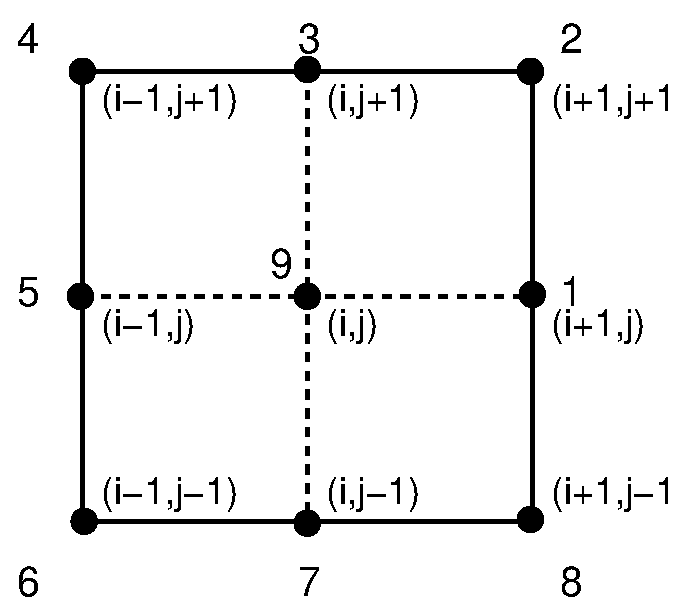
\includegraphics[scale=0.3]{./tex_plot/stencil.eps}
  \caption{Geometry for the 9 point stencil}
   \label{fig:stencil}
\end{figure}
%
The values at half grid points e.g. $(i+\frac{1}{2},j)$ are determined
by averaging the values of the adjacent grid points.
%
\begin{equation}
 \Sigma_{\phi \phi}^T(i+\frac{1}{2},j) = \frac{1}{2}
   \bigl[ \Sigma_{\phi \phi}^T(i+1,j) +  \Sigma_{\phi \phi}^T(i,j) \bigr]
\end{equation}
%
Accordingly values at $(i-\frac{1}{2},j)$, $(i,j+\frac{1}{2})$ and
$(i,j-\frac{1}{2})$ can be calculated. The difference at half points
in latitude and longitude e.g.  $(i+\frac{1}{2},j+\frac{1}{2})$
is also resolved by veraging the values of the adjacent grid 
points which leads to e.g.
%
\begin{equation}
 \Phi(i+\frac{1}{2},j+\frac{1}{2}) - \Phi(i+\frac{1}{2},j-\frac{1}{2}) = \frac{1}{4}
   \bigl[ \Phi(i+1,j+1) -\Phi(i+1,j-1) + \Phi(i,j+1)- \Phi(i,j-1) \bigr]
\end{equation}
%
